\section{GIÁ TRỊ LỚN NHẤT - NHỎ NHẤT CỦA HÀM SỐ}

\subsection{LÝ THUYẾT CẦN NHỚ}
Cho hàm số $y=f(x)$ xác định trên tập $\mathscr{D}$. Ta có
\immini{\begin{itemize}
		\item[\ding{172}] $M$ là giá trị lớn nhất của hàm số nếu $\heva{&f(x) \le M,\forall x \in \mathscr{D}\\& \exists x_0 \in \mathscr{D}: f(x_0)=M.}$\\
		Kí hiệu \fbox{$\displaystyle\max_{x \in \mathscr{D}}f(x)=M$}
		\vskip 0.5cm
		\item[\ding{173}] $n$ là giá trị nhỏ nhất của hàm số nếu $\heva{&f(x) \ge n,\forall x \in \mathscr{D}\\& \exists x_0 \in \mathscr{D}: f(x_0)=n.}$\\
		Kí hiệu \fbox{$\displaystyle\min_{x \in \mathscr{D}}f(x)=n$}
\end{itemize}
}{
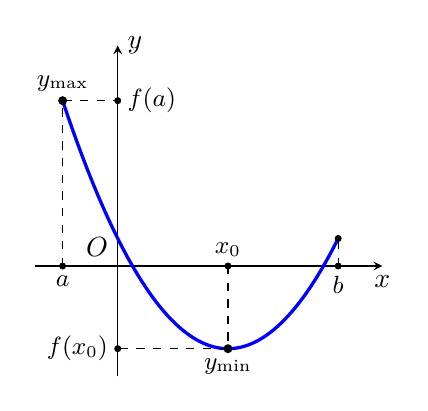
\begin{tikzpicture}[smooth,samples=300,scale=0.7,>=stealth]
	\draw[->] (-1.5,0)--(4.8,0) node[below]{$x$};
	\draw[->] (0,-2)--(0,4) node[right]{$y$};
	\draw (0,0) node[above left]{$O$};
	\draw[line width = 1.2pt,domain=-1:4,blue] plot(\x,{0.5*((\x)^2-4*(\x)+1)});
	\draw[fill=black] (-1,0) circle(1.5pt) (-1,3) circle(2pt) (0,3) circle(1.5pt) (0,-1.5) circle(1.5pt) (2,0) circle(1.5pt) (2,-1.5) circle(2pt) (4,0) circle(1.5pt) (4,0.5) circle(1.5pt);
	\draw[dashed] (-1,0)node[below]{\small$a$}--(-1,3)--(0,3)node[right]{\small$f(a)$} (2,0)node[above]{\small$x_0$}--(2,-1.5)--(0,-1.5)node[left]{\small$f(x_0)$}
	(4,0)node[below]{\small$b$}--(4,0.5);
	\node[above] at (-1,3) {\small $y_{\max}$};
	\node[below] at (2,-1.5) {\small $y_{\min}$};
\end{tikzpicture}}
\begin{note}
	\begin{itemize}
		\item [\ding{172}] Khi yêu cầu tìm max min của hàm số mà không nói rõ xét trên tập nào, thì ta hiểu là tìm max min trên miền xác định của hàm số đó.
		\item [\ding{173}] Để tìm max min của hàm số $y=f(x)$ trên miền $\mathscr{D}$, ta thường lập bảng biến thiên của hàm số $y=f(x)$ trên $\mathscr{D}$. Từ bảng biến thiên, ta kết luận:
		\begin{itemize}
			\item [$\bullet$] Điểm ở vị trí cao nhất $\longrightarrow$ Kết luận max;
			\item [$\bullet$] Điểm ở vị trí thấp nhất $\longrightarrow$ Kết luận min.
		\end{itemize}
		\item [\ding{174}] Để tìm max min của hàm số $y=f(x)$ trên đoạn $[a;b]$ (\textit{$f(x)$ liên tục trên đoạn $[a ; b]$ và có đạo hàm trên $(a ; b)$ (có thể trừ một số hữu hạn các điểm) và $f^{\prime}(x)=0$ chỉ tại một số hữu hạn các điểm trong $(a ; b)$}), thì ta có thể giải như sau:
		\begin{itemize}
			\item [$\bullet$] Giải $f'(x)=0$ tìm các nghiệm $x_0 \in (a;b)$; 
			\item [$\bullet$] Tìm các điểm $x_i\in (a;b)$ mà tại đó đạo hàm không xác định (nếu có).
			\item [$\bullet$] Tính toán $f(a)$, $f(x_0)$, $f(x_i)$, $f(b)$ \quad ($\star$)
			\item [$\bullet$]  Gọi $M$, $n$ lần lượt là số lớn nhất và số nhỏ nhất của các kết quả tính toán ở bước ($\star$) thì
			$$M=\displaystyle\max_{[a;b]}f(x); \quad n=\displaystyle\min_{[a;b]}f(x)$$
		\end{itemize}
	\item [\ding{175}] Ta có thể dùng các bất đẳng thức có sẵn để đánh giá biểu thức cần tìm max, min. 
	\begin{itemize}
		\item [$\bullet$] Bất đẳng thức Cô-si cho hai số không âm $a$, $b$:
		$$a+b \ge 2\sqrt{ab}$$
		Dấu "=" xảy ra khi $a=b$.
		\item [$\bullet$]  Bất đẳng thức Cô-si cho ba số không âm $a$, $b$, $c$:
		$$a+b +c\ge 3\sqrt[3]{abc}$$
		Dấu "=" xảy ra khi $a=b=c$.
	\end{itemize}
	\end{itemize}
\end{note}
